\chapter{Technik}
\label{cha:technik}
Das folgende Kapitel beschäftigt sich mit der bei diesem Projekt einzusetzenden Technik. Wie der Titel dieser Arbeit bereits verdeutlicht, soll dieses Projekt mit Hilfe von Wearable-Computern umgesetzt werden. In den folgenden Unterkapiteln sollen darüber hinaus weitere Gerätetypen dargestellt und miteinander verglichen werden. Die für diese Arbeit verwendete \emph{Vuzix M100} Smartglass soll bewertet werden. Beim Vergleich der Gerätetypen wird nur die Hardware verglichen, die Software wird später definiert und im Rahmen dieses Projektes entwickelt. Dieses Kapitel soll sicherstellen, dass die eingesetzte Technik für die Erfüllung der Ziele am besten geeignet ist.\\

Beim Vergleich der Hardware wird insbesondere auf die definierten Ziele\footnote{Siehe Kapitel \ref{sec:zieldefinition} \nameref{sec:zieldefinition}} eingegangen, die mit Hilfe dieses Projektes in Verbindung mit der hier ausgewählten Hardware erreicht werden sollen. Außerdem wird hauptsächlich auch auf die Usability der Geräte eingegangen, die Voraussetzung für eine effektive und effiziente Arbeit mit dem Produkt ist. 

\section{Gerätetypen}
\label{sec:geraete}
In Kapitel \ref{cha:bedarfsanalyse} \nameref{cha:bedarfsanalyse} wurde der Bedarf an elektronischer Hilfe bei der Warenannahme/-einräumung erläutert, um auf dem Markt langfristig wettbewerbsfähig zu bleiben. Die Warenannahme und -einräumung findet an verschiedenen Stellen der Filiale statt und das sowohl im Lager- als auch im Kundenbereich. Feststehende große Gerätschaften sind somit nicht praktikabel und werden bereits ausgeschlossen. Voraussetzung sind somit mobile Gerätetypen mit aktuellen Schnittstellen \bzw Verbindungsmöglichkeiten, die eine reibungslose Integration in jedes Firmennetzwerk ermöglichen.\\
Aus diesen Anforderungen lassen sich folgende Gerätetypen ableiten:
\begin{itemize}
	\item Laptop
	\item Tablet-PC
	\item Tablet
	\item Smartphone
	\item Wearable Computer
\end{itemize}
Laptops bieten sehr viel Rechenleistung bei einem -- gegenüber klassischen Tower-Computern -- vergleichsweise geringem Gewicht. Gegenüber den anderen Gerätetypen sind diese bei weitem leistungsstärker und bieten sehr viele Anschlussmöglichkeiten, ohne an die Leistungsgrenzen zu stoßen. Diese Rechenleistung ist in diesem Projekt aber nicht erforderlich, da die Anwendung keine großartigen \acs{3D}-Grafikberechnungen durchführen muss und z.B. keine aufwändigen mathematischen Formeln gelöst werden müssen. Ein Laptop ist jedoch deutlich unhandlicher als die anderen Gerätetypen und benötigt durch die Beschaffenheit der Eingabegeräte (Tastatur und Maus) mehr Aufmerksamkeit des Benutzers. Augmented Reality lässt sich durch einen Laptop außerdem nicht umsetzen, da die Nutzung beide Hände benötigt -- ein Einräumen der Ware und gleichzeitiges Benutzen des Laptops, der dem Anwender Hinweise auf den Warenstandort gibt, ist nicht möglich.\\

Tablet-PCs\footnote{Tablet-PCs werden in dieser Arbeit als Computer mit Touchbildschirm definiert, die mit bestimmter Technik durch den Benutzer schnell in ein Tablet-ähnliches Gerät verwandelt werden können.} \bzw Tablets haben eine geringere Leistungsfähigkeit als Laptops, haben aber für dieses Projekt den Vorteil, dass sie deutlich handlicher sind. Darüber hinaus besitzen aktuelle Tablets gängige Verbindungsmöglichkeiten und sind daher einfach in das Netzwerk integrierbar. Durch eine Kamera auf der Rückseite wäre außerdem das Umsetzen von Augmented Reality möglich. Bei einem Tablet ist jedoch zu beachten, dass die Bedienung weiterhin zwei Hände benötigt und das Einräumen \bzw die Annahme der Ware nicht parallel stattfinden kann.\\

Ein aktuelles Smartphone besitzt inzwischen ähnliche Leistungsmerkmale wie ein Tablet mit den selben Verbindungs- und Eingabemöglichkeiten. Da ein Smartphone mit einer Bildschirmdiagonale von maximal 5 bis 6 Zoll nochmals deutlich kleiner als ein Tablet ist und sowohl durch eine Hand bedienbar ist, als auch schnell und einfach (\zB in der Hosentasche) verstaut werden kann, eignet es sich besser für \acs{SMAR} als die anderen Technologien. Der Benutzer kann gleichzeitig eine App auf dem Smartphone bedienen, darüber Produkte einfach scannen und das Produkt einräumen. Der Mehrwert gegenüber der Warenannahme mit Setzliste ist deutlich gegeben. Darüber hinaus ist die Bedienung einer Smartphone-App vielen Benutzern bekannt (Stand Februar 2015: 45,6 Millionen Menschen in Deutschland sind Smartphone-Nutzer), was hier die Einarbeitungszeit verkürzt.\footnote{\citep{statista_smartphone}} Im Kontext dieses Projektes sind Smartphones ausschließlich für Augmented Reality nicht geeignet, da sie dafür ständig in der Hand gehalten und auf ein Regal ausgerichtet werden müssen -- eine Tätigkeit, die wenig ergonomisch ist.\\

Als \emph{Wearable Computer} werden Computer bezeichnet, die am Körper getragen werden können und dabei Körperbewegungen nicht einschränken, das heißt die Hände sollen zu jeder Zeit frei sein und höchstens bei direkter Bedienung des Gerätes belegt sein. Die derzeit verbreiteten \bzw verwendeten Wearable Computer können in zwei Kategorien unterteilt werden:
\begin{enumerate}
	\item Smartwatches
	\item Smartglasses
\end{enumerate}
Smartwatches sind Armbanduhren mit einem Touchbildschirm, die durch die Verbindung mit dem Smartphone das Anzeigen von Kalender-, Nachrichten-, Navigations- und weiteren Informationen erlauben. Da die Smartwatches ein sehr kleines Display und in der Regel keine Kamera besitzen, sind diese für die Warenannahme und Augmented Reality nicht geeignet.\\
Smartglasses sind hingegen Computer, die in eine Brille integriert werden oder über ein Bügel vor das Auge geschoben werden können (einem Headset ähnlich). Die Bedienung über Knöpfe soll hier vermieden und die Bedienung per Sprache und Gesten präferiert werden. Darüber hinaus ist ein Ziel von Smartglasses, dass die Brillen \bzw die Apps, die auf den Smartglasses laufen, mit Hilfe von Kameras und Augmented Reality in die Umwelt integriert werden. Diese Technologie befindet sich aktuell noch in der Entwicklungsphase und ist daher noch nicht ausgereift. Dennoch eignet sich diese Technologie für die Bedürfnisse, die an dieses Projekt gekoppelt sind, optimal. Zur Bedienung muss kein Gerät in der Hand gehalten werden, sodass diese frei für die Erledigung der eigentlichen Aufgabe sind; außerdem befindet sich das Display jederzeit im Blick und ermöglicht somit die Warenannahme \bzw -einräumung und das Abrufen der dafür notwendigen Informationen (wie \zB Regalplatz) gleichzeitig.\\

Das Benutzen von Wearable Computern, im Speziellen von Smartglasses, ist somit sinnvoll und wird, nach Einarbeitung der Anwender, voraussichtlich erheblichen Mehrwert erzeugen. Für eine schnelle Bearbeitung von kleineren Aufgaben sollte die App allerdings auch für das Smartphone ohne Augmented Reality zur Verfügung stehen. Dies ermöglicht \zB eine schnelle Unterstützung des Kunden bei der Suche eines Produktes.

Die folgende Abbildung zeigt den zusammengefassten Vergleich der verschiedenen Gerätetypen auf:
\begin{figure}[H]
	\centering
	{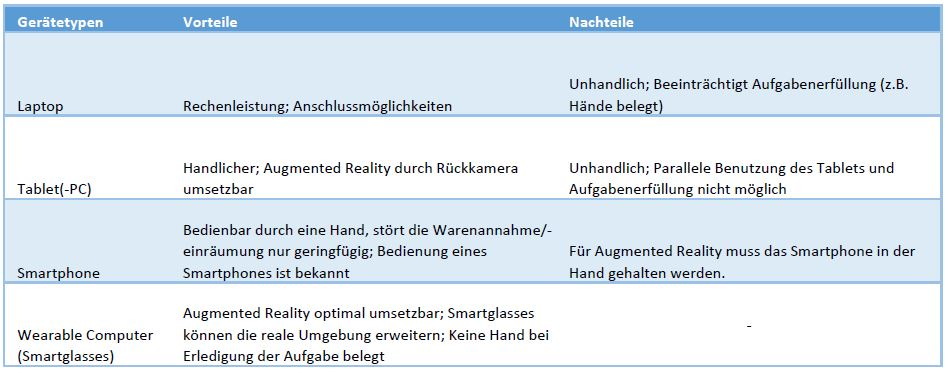
\includegraphics[width=\textwidth]{Bilder/device_comparison.jpg}}
	\caption{Vergleich Gerätetypen}
	\label{fig:role_web}
\end{figure}

\section{Vuzix M100}
\label{sec:vuzix}
Eine Betrachtung der verschiedenen Möglichkeiten zeigt, wie bereits beschrieben, dass eine Datenbrille besondere Vorteile aufweist. Für die Betrachtung und Bedienung des Gerätes ist keine freie Hand nötig, sodass das Einräumen in ein Regal nicht behindert wird. Für das in dieser Studienarbeit behandelte Projekt \glqq Shelf-Management mit Hilfe von Augmented Reality\grqq\ stand die \glqq Vuzix M100 Smart Glasses\grqq\ Datenbrille zur Verfügung.

\subsection{Technische Daten}
Die Datenbrille von Vuzix ist mit einem 1 \ac{GB} großen LPDDR2 400 \ac{MHz} Arbeitsspeicher und einem OMAP4430 Prozessor ausgestattet, der Dual-Core Prozessor basiert auf der \acs{ARM}-Architektur und taktet mit bis zu 1 \ac{GHz}.\footnote{\citep{omap4430}} Die 4 \ac{GB} Flash-Speicher können durch den Micro-\acs{SD} Kartenslot erweitert werden, der eine Kartengröße bis 32 \ac{GB} unterstützt. Betrieben wird dieses System mit Android Ice Cream Sandwich (Version 4.0).\footnote{\citep{vuzixm100}}\\

Das Display hat eine Auflösung von 432 x 240 Pixel (Breite mal Höhe) bei einem Breitbild-Seitenverhältnis von 16:9.\footnote{\citep{wqvga}} Außerdem bietet es eine Farbtiefe von 24 bit. Durch die Wölbung des Displays um 15 Grad, wirkt das Display der getragenen Brille –- laut Hersteller -- wie ein Monitor mit einer Bilddiagonale von 4 Zoll.\footnote{circa 10 \ac{cm}}\\

Die 5 Megapixel Kamera nimmt Bilder und Videos ebenfalls im 16:9 Seitenverhältnis auf. Videos werden in Full-\acs{HD} Auflösung aufgenommen (1920 x 1080 Pixel). Allerdings besitzt die Kamera weder einen Blitz noch ein LED-Licht zur Verbesserung von schlechten Lichtverhältnissen.\\

Das Gerät kann über verschiedenste Wege bedient werden. Auf der Seite befinden sich 4 Kontrollknöpfe, die zum Ein- und Ausschalten, sowie für das Bewegen und Selektieren im Menü benutzt werden können. Das Mikrofon ermöglicht die Kontrolle per Sprache, entsprechende \glqq Nuance Voice Control\grqq -Software wird über das Betriebssystem geliefert. Das \glqq Noise Cancelling Microphone\grqq\ nimmt Umgebungsgeräusche auf und filtert sie aus dem Eingang des Spracherkennungs-Mikrofons raus. Dadurch ist die Stimme auch in lauten Umgebungen deutlicher und die Spracherkennung/-kontrolle funktioniert auch bei vielen Hintergrundgeräuschen. Außerdem ist es möglich, das Gerät über Gesten (wie z.B. Nicken, Kopf nach links/rechts schwenken) durch die eingebaute \glqq 3 DOF Gesture Engine\grqq\ zu steuern.\footnote{\citep{vuzixm100}}\\

Die Verbindung zwischen der Vuzix M100 Datenbrille und anderen Geräten oder Netzwerken kann drahtlos über WLAN im Standard 802.11b/g/n oder über Bluetooth 4.0 hergestellt werden. Drahtgebunden kann das Gerät über \ac{USB} verbunden werden. Über die \ac{USB}-Schnittstelle können darüber hinaus Softwareupdates eingespielt und das Gerät aufgeladen werden.\footnote{\citep{vuzixm100}}\\
Im \ac{WLAN} erreicht das Gerät Datenübertragungsraten von maximal 150Mbit/s, dies entspricht dem IEEE802.11n Standard auf dem 2.4GHz Frequenzband.\footnote{\citep{uebertragungsgeschwindigkeit}} Dies reicht für das Aufrufen von Webseiten, Übertragen von Bildern mit einer Auflösung von 432 x 240 Pixel (Breite x Höhe), sowie für das Übertragen weiterer Informationsdaten zur Bestimmung der Position einer Ware binnen weniger Sekunden aus.\\
Da Bluetooth 4.0 eine maximale Reichweite von 100 Metern erreichen kann (und das auch nur theoretisch, gängig sind Reichweiten von ca. 10 - 50 Metern)\footnote{\citep{bluetooth}} und eine Übertragungsrate von nur ca. 1-2 Mbit/s erreicht, eignet es sich nicht zur Datenübertragung von Regalbildern oder komplexen Positionsbeschreibungen und Datenbankabfragen nach einem Produkt. Bluetooth eignet sich hingegen gut für die Verbindung zu Host-Systemen zur externen Steuerung der Datenbrille\footnote{Voraussetzung ist ein Android-Handy mit entsprechender App} und zur Anbindung externer Geräte, wie z.B. einem Bluetooth Barcode-Scanner.

\subsection{Bewertung}
Die Leistung der Vuzix M100 Smartglasses ist durch das Datenblatt bereits ausführlich beschrieben und ist sowohl für das Android-Bertriebssystem als auch für dieses Projekt zufriedenstellend. Verbindungen per \ac{WLAN} und Bluetooth konnten ohne Probleme hergestellt werden und liefen stabil. Die Verbindung in ein ausreichend gedecktes \ac{WLAN}-Firmennetzwerk sollte daher ohne Probleme funktionieren.\\

Doch bei diesem Projekt steht die Leistung des Gerätes nicht ausschließlich im Vordergrund. Ein besonderes Augenmerk sollte auf den Tragekomfort und die Usability gelegt werden. Diese wird in diesem Kapitel anhand von subjektiven Wahrnehmungen der Entwickler beschrieben.\\

Besonders die Vorteile dieses Gerätetyps sind nochmal hervorzuheben. Während alle anderen Gerätetypen bei weiteren Aufgaben behindernd oder störend wirken, ist bei den Smartglasses keinerlei Beeinträchtigung zu erkennen. Die Smartglass benötigt für das Mitführen des Gerätes und das Einsehen von Informationen keine Hände und beeinträchtigt die Bewegungsfreiheit nicht. Der Bügel \bzw die Brille müssen beim Aufsetzen sehr genau justiert werden, damit das Display vollkommen eingesehen werden kann. Dies dauerte in der Anwendung oft mehrere Augenblicke und wurde als noch nicht ausgereift empfunden, doch sobald das Display korrekt saß, verharrte es in dieser Position und es bedurfte nur selten einer weiteren Korrektur. Außerdem wurde die Brille auch beim Betrachten der Umwelt nicht als störend oder einschränkend empfunden.\\

Die Produkterkennung findet selbstverständlich über die entsprechenden Barcodes statt, daher musste zuerst überprüft werden, wie diese am besten in die App übertragen werden können. Die Smartglass eröffnet dabei zwei Möglichkeiten:
\begin{itemize}
	\item Erfassen von Barcodes über einen externen, per Bluetooth verbundenen Barcode-Scanner.
	\item Erfassen von Barcodes über die eingebaute Kamera in Verbindung mit einer entsprechenden Android Library.
\end{itemize}
Der Bar-Code-Scanner hat den entscheidenden Nachteil, dass der Anwender ein weiteres Gerät in der Hand halten muss, welches die Bewegungsfreiheit wiederum einschränkt. Die Erfassung von Barcodes über die Kamera konnte über eine vorinstallierte App getestet werden. Dies funktionierte schnell (unter 2 Sekunden) und auch bei schlechteren Lichtverhältnissen zuverlässig. Für das Projekt, welches aktuell\footnote{Stand: Mai 2015} noch keinen geplanten Live-Einsatz hat, war dies daher ausreichend und zufriedenstellend. Darüber hinaus war die Erfassung des Barcodes somit allein durch Bewegen des Kopfes in Produktrichtung möglich.\\

Ein weiterer wichtiger Punkt ist die Bedienung und die Navigation durch das Betriebssystem \bzw die App. Die wenigen Knöpfe sind am Ohr schnell zu finden und besitzen einen angenehmen Druckpunkt. Durch eine leicht verzögerte Reaktion wirkt die Bedienung oft nicht vollständig flüssig und erzeugt gegenüber dem Anwender das Gefühl, die Eingabe erneut ausführen zu müssen. Auch die Spracherkennung ist noch nicht vollständig ausgereift und benötigt oft ein erneutes Einsprechen des Befehls, darüber hinaus wird zur Zeit ausschließlich die englische Sprache unterstützt.\\

Der entscheidende Negativmerkmal der Vuzix M100 ist jedoch das Display. Neben der langwierigen Justierung der Brille, bis das Display vollständig einzusehen ist, fällt vor allem jedoch die geringe Auflösung und die Größe des Displays negativ auf. Werden beim Programmieren TextViews\footnote{Reservierte Felder für die Ausgabe von Textinformationen} mit der Größe SMALL (klein) ausgewählt, so kann dies auf einem Smartphone-Display gut eingesehen werden, auf der Smartglass ist dies jedoch nicht oder nur sehr schwer erkennbar. Auf dem Display können daher leider nur sehr wenige Informationen oder kleine Teile eines Regals angezeigt werden. Das ist für den Produktiveinsatz nicht sehr praktikabel.\\

Trotz der in diesem Kapitel beschriebenen negativen Punkte ist zu beachten, dass es sich bei der Smartglass und bei diesem Projekt (\acs{SMAR}) noch um Prototypen handelt, für die es noch keine geplanten Live-Einsätze gibt. Die Vorteile gegenüber den anderen vorgestellten Gerätetypen müssen außerdem berücksichtigt werden, sodass ein Mehrwert durch das Einsetzen der Technologie bereits erzeugt wird, der aber noch verbesserungswürdig ist.
Die mögliche zukünftige Verwendung wird im Kapitel \ref{cha:ausblick} (\nameref{cha:ausblick}) näher beschrieben.